\documentclass[a4paper,11pt,french]{article}
\usepackage[margin=2cm]{geometry}
\usepackage[thinfonts,latinmath]{uglix2}
\nouveaustyle
\pagestyle{empty}
\begin{document}
\titre{Corrigé de l'évaluation}{\premiere}{27/09/2022}

\begin{exercice}[ (8 points)]
	Résoudre les inéquations suivantes :
	\begin{multicols}{3}
		\begin{enumerate}[\bfseries 1.]
			\item 	$5x-2> 8x+31$
			\item 	$(2x+1)(3x-2)\geqslant0$
			\item	$\dfrac{-5x-2}{-7x+8}\geqslant0$
		\end{enumerate}
	\end{multicols}
\end{exercice}

\begin{exercicecorrection}
	\begin{enumerate}[\bfseries 1.]
		\item 	\begin{tabbing}
			$5x-2> 8x+31 \quad$		\=	$\Leftrightarrow\quad -3x>33 $\\
			\>	$\Leftrightarrow\quad x<-11$
		\end{tabbing}
		$\mathcal{S_1}=\oio{-\infty}{-11}$
		\item 	$(2x+1)(3x-2)\geqslant0$\\[.5em]
		On a le tableau de signes suivant :
		\begin{center}
			\begin{tikzpicture}
				\tkzTabInit[color,lgt=5,espcl=3]
				{$x$ /1 , signe de $2x+1$ /1, signe de $3x-2$ /1, signe de $(2x+1)(3x-2)$ /1}
				{$-\infty$, $-\dfrac{1}{2}$ , $\dfrac{2}{3}$, $+\infty$ }
				\tkzTabLine{,-, z, + , t , +,}
				\tkzTabLine{,-, t, - , z , +,}
				\tkzTabLine{,+, z, - , z, +,}
			\end{tikzpicture}
		\end{center}
		D'où $\mathcal{S_2}=\oif{-\infty}{-\dfrac{1}{2}}\cup\fio{\dfrac{2}{3}}{+\infty}$.
		\item	$\dfrac{-5x-2}{-7x+8}\geqslant0$\\[.5em]
		On a le tableau de signes suivant :
		\begin{center}
			\begin{tikzpicture}
				\tkzTabInit[color,lgt=5,espcl=3]
				{$x$ /1 , signe de $-5x-2$ /1, signe de $-7x+8$ /1, signe de $\dfrac{-5x-2}{-7x+8}$ /1}
				{$-\infty$, $-\dfrac{2}{5}$ , $\dfrac{8}{7}$, $+\infty$ }
				\tkzTabLine{,+, z, - , t , -,}
				\tkzTabLine{,+, t, + , z , -,}
				\tkzTabLine{,+, z, - , d, +,}
			\end{tikzpicture}
		\end{center}
	D'où $\mathcal{S_3}=\oif{-\infty}{-\dfrac{2}{5}}\cup\oio{\dfrac{8}{7}}{+\infty}$
	\end{enumerate}
\end{exercicecorrection}




\begin{exercice}[ (8 points)]
	\begin{minipage}{9.5cm}
		\begin{enumerate}[\bfseries 1.]
			\item 	Donner sans justifier les équations des droites $(d_1)$ et $(d_2)$.
			\item 	On considère $f_1$ et $f_2$ les fonctions représentées par $(d_1)$ et $(d_2)$.\\
			Résoudre graphiquement $f_1(x)=f_2(x)$.
			\item	On considère la fonction affine $f$ telle que $f(1)=6$ et $f(7)=1$.\\
			Déterminer par le calcul une expression algébrique de $f$.
			\item	Le point $\pc{K}{-10}{65}$ appartient-il à $(d)$, la droite représentative de $f$ ?
		\end{enumerate}
	\end{minipage}
	\begin{minipage}{7cm}
		\begin{flushright}
			\def\xmin{-2} \def\ymin{-5}\def\xmax{9}\def\ymax{4}
			\def\F{-1/3*\x+2}\def\G{2/7*\x-3}
			\begin{tikzpicture}[scale=.6]
				\clip (\xmin,\ymin) rectangle (\xmax,\ymax);
				\draw[fill = white] (\xmin,\ymin) rectangle (\xmax,\ymax);
				\reperevl{\xmin}{\ymin}{\xmax}{\ymax}
				\draw[thick,domain=\xmin:\xmax,smooth,variable=\x] plot ({\x},{\F});	
				\draw[thick,domain=\xmin:\xmax,smooth,variable=\x] plot ({\x},{\G});
				\draw (0,2)\ball (0,-3)\ball (6,0)\ball(7,-1)\ball;	
				\draw (-1.2,2.5) node [above]{$(d_1)$};	
				\draw (-1.2,-3.5) node [below]{$(d_2)$};	
			\end{tikzpicture}
		\end{flushright}
		
	\end{minipage}
\end{exercice}

\begin{exercicecorrection}
	\begin{enumerate}[\bfseries 1.]
		\item 	$(d_1):y=-\dfrac{1}{3}x+2 \quad$ et $(d_2):y=\dfrac{2}{7}x-3$.
		\item 	La solution de l'équation $f_1(x)=f_2(x)$ est l'abscisse du point d'intersection des droites $(d_1)$ et $(d_2)$, soit $8$.
		\item	$f$ est affine. Il existe donc deux réels $m$ et $p$ tels que pour tout $x\in\R, \ f(x)=mx+p$.
		\begin{multicols}{2}
			\textbf{Déterminons $m$ :}
			\begin{tabbing}
				$m$ 	\=  $=\dfrac{f(7)-f(1)}{7-1} $\\[.5em]
				\>  $= \dfrac{1-6}{6}$\\[.5em]
				\>	$= -\dfrac{5}{6}$
			\end{tabbing}
			D'où pour tout $x\in \R, f(x)=-\dfrac{5}{6}x+p$.
			
			\textbf{Déterminons $p$ :}
			\begin{tabbing}
				$f(1)=6 \quad$		\=	$\Leftrightarrow\quad -\dfrac{5}{6}\times1+p=6$\\
				\>	$\Leftrightarrow\quad p=6+\dfrac{5}{6} $\\
				\>	$\Leftrightarrow\quad p=\dfrac{41}{6}$
			\end{tabbing}
			D'où pour tout $x\in \R, f(x)=-\dfrac{5}{6}x+\dfrac{41}{6}$.
		\end{multicols}
		\item	On cherche à vérifier si $f(-10)=65$.
		\begin{tabbing}
			$f(-10)$ 	\=  $=-\dfrac{5}{6}\times(-10)+\dfrac{41}{6} $\\[.5em]
			\>  $= \dfrac{50}{6}+\dfrac{41}{6}$\\[.5em]
			\>	$= \dfrac{91}{6}$\\[.5em]
			\>	$\neq	\dfrac{390}{6}=65$
		\end{tabbing}
		les coordonnées de $K$ ne sont pas solution de l'équation de $(d)$ donc $K$ n'appartient pas à $(d)$.
	\end{enumerate}
\end{exercicecorrection}

\begin{exercice}[ (8 points)]
	\begin{enumerate}[\bfseries 1.]
		\item 	Démontrer que, pour tout $x$ réel différent de $5$, $\quad \dfrac{x}{2x-10}-2=\dfrac{-3x+20}{2x-10}$.\\
		En déduire les solutions de $\quad \dfrac{x}{2x-10}\geqslant2$.
		\item 	Résoudre l'inéquation $\quad \dfrac{1-4x}{x-3}<4$.
	\end{enumerate}
\end{exercice}

\begin{exercicecorrection}
	\begin{multicols}{2}
		\begin{enumerate}[\bfseries 1.]
			\item 	Soit $x\in\R\backslash\left\{5\right\}$.
			\begin{tabbing}
				$\dfrac{x}{2x-10}-2$ 	\=  $=\dfrac{x}{2x-10} - \dfrac{2(2x-10)}{2x-10} $\\[.5em]
				\>  $= \dfrac{x}{2x-10} - \dfrac{4x-20}{2x-10}$\\[.5em]
				\>	$= \dfrac{x-(4x-20)}{2x-10}$\\[.5em]
				\>	$= \dfrac{x-4x+20}{2x-10}$\\[.5em]
				\>	$= \dfrac{-3x+20}{2x-10}$
			\end{tabbing}
			On a donc :
			\begin{tabbing}
				$\dfrac{x}{2x-10}\geqslant2 \quad$		\=	$\Leftrightarrow\quad \dfrac{x}{2x-10}-2\geqslant0 $\\[.5em]
				\>	$\Leftrightarrow\quad  \dfrac{-3x+20}{2x-10}\geqslant0$
			\end{tabbing}
			On peut donc écrire le tableau de signes :\\[.5em]
			%\begin{center}
				\begin{tikzpicture}
					\tkzTabInit[color,lgt=3.7,espcl=1]
					{$x$ /1 , signe de $-3x+20$ /1, signe de $2x-10$ /1, signe de $\dfrac{-3x+20}{2x-10}$ /1}
					{$-\infty$, $5$ , $\dfrac{20}{3}$, $+\infty$ }
					\tkzTabLine{,+, t, + , z , -,}
					\tkzTabLine{,-, z, + , t , +,}
					\tkzTabLine{,-, d, + , z, -,}
				\end{tikzpicture}\\[.5em]
			%\end{center}
			D'où $\mathcal{S_1}=\oif{5}{\dfrac{20}{3}}$.\columnbreak
			\item	Soit $x\in\R\backslash\left\{3\right\}$.
			\begin{tabbing}
				$\dfrac{1-4x}{x-3} <4 \quad$		\=	$\Leftrightarrow\quad \dfrac{1-4x}{x-3} -4 <0 $\\[.5em]
				\>	$\Leftrightarrow\quad  \dfrac{1-4x}{x-3} -\dfrac{4(x-3)}{x-3} <0$\\[.5em]
				\>	$\Leftrightarrow\quad	\dfrac{1-4x}{x-3} - \dfrac{4x-12}{x-3} <0$\\[.5em]
				\>	$\Leftrightarrow\quad	\dfrac{1-4x-(4x-12)}{x-3} <0$\\[.5em]
				\>	$\Leftrightarrow\quad	\dfrac{1-4x-4x+12}{x-3} <0$\\[.5em]
				\>	$\Leftrightarrow\quad	\dfrac{-8x+13}{x-3} <0$
			\end{tabbing}
			On peut donc écrire le tableau de signes :\\[.5em]
			%\begin{center}
				\begin{tikzpicture}
					\tkzTabInit[color,lgt=3.7,espcl=1]
					{$x$ /1 , signe de $-8x+13$ /1, signe de $x-3$ /1, signe de $\dfrac{-8x+13}{x-3}$ /1}
					{$-\infty$, $\dfrac{13}{8}$ , $3$, $+\infty$ }
					\tkzTabLine{,+, z, - , t , -,}
					\tkzTabLine{,-, t, - , z , +,}
					\tkzTabLine{,-, z, + , d, -,}
				\end{tikzpicture}\\[.5em]
			%\end{center}
			D'où $\mathcal{S_2}=\oio{-\infty}{\dfrac{13}{8}}\cup\oio{3}{+\infty}$.
		\end{enumerate}
	\end{multicols}
	
\end{exercicecorrection}

\newpage
\begin{exercice}[ (2 points + 4 points bonus)]
	Soit $f$ une fonction affine définie pour tout $x\in \R$ par $\ f(x)=mx+p$.\\
	On appelle $f^2$ la fonction définie pour tout $x\in\R$ par $\ f^2(x)=f(f(x))$.\\
	On généralise cette notation pour $n\in\N$ : \ pour tout $x\in\R, \quad f^{n+1}(x)=f(f^n(x)) \quad$ et $\quad f^0(x)=x$.
	\begin{enumerate}[\bfseries 1.]
		\item 	Vérifier que pour $n=1, n=2$ et $n=3$, les fonctions $f^n$ sont affines.
		\item 	Quelle conjecture peut-on faire sur le taux d'accroissement et l'ordonnée à l'origine de $f^n$ pour $n\in\N^*$ ?
		\item	Déterminer une fonction affine $f$ vérifiant la propriété suivante : \og Il existe un entier $n>1$ tel que $f^n(x)=2048x-2047$.
	\end{enumerate}
\end{exercice}

\end{document}
